\documentclass[a4paper,12pt]{article}
\usepackage[utf8]{inputenc} % para acentos y eñes
\usepackage[spanish]{babel} % en español
\usepackage{verbatim} % para comentarios multilinea
\usepackage{moreverb} % para verbatim con tabs
\usepackage{graphicx} % para imagenes
\usepackage{hyperref} % para links web e intradocumento
\usepackage{caption} % para varias imagenes en una linea
\usepackage{subcaption} % para varias imagenes en una linea
\usepackage{url}

% \usepackage{times} % tipo de letra de periodico
\renewcommand{\familydefault}{\sfdefault} % letras sin serifa

%opening
\title{Perfiles SAML}
\author{Práctica 1 de Seguridad 2012-13}
\date{}



\begin{document}

\maketitle

\begin{center}
Leandro J. Guillén Moreno 48510228P leandrojesus.guillen@um.es
\end{center}

% \newpage % salto de página manual
\tableofcontents

%%%%%%%%%%%%%%%%%%%%%%%%%%%%%%%%%%%%%%%%%%%%%%%%%%%
\newpage
\section{Diseño}

El escenario se compone de tres entidades (ver figura \ref{fig:escenario}):
\begin{itemize}
 \item Service Provider.
 \item Service Provider 2.
 \item Identity Provider.
\end{itemize}

\begin{figure}[h!]
\centering
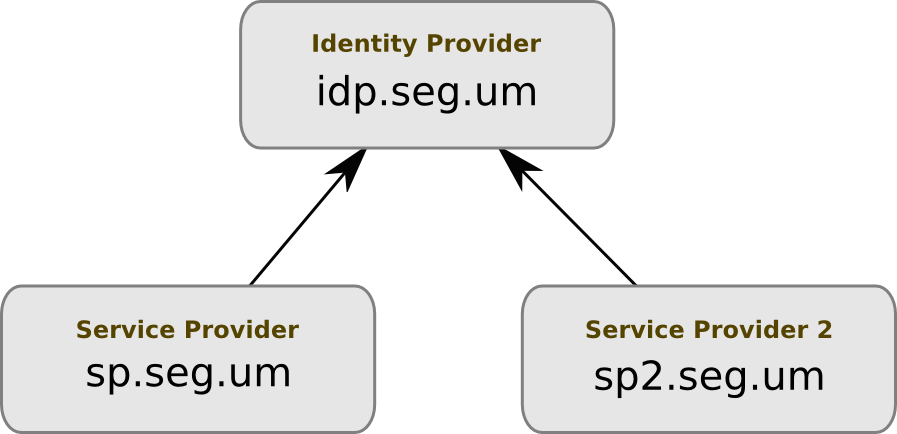
\includegraphics[width=0.7\textwidth]{img/escenario}
\caption{Escenario de la práctica y relaciones de confianza.}
\label{fig:escenario}
\end{figure}

Cada una de las máquinas ha sido montada en una máquina virtual con VirtualBox (ver figura \ref{fig:vbox}). Es requisito indispensable que los nombres de dominio indicados en la figura \ref{fig:escenario} sean resolubles en el cliente. Por ejemplo, configurándolos en el fichero \emph{/etc/hosts} en linux.

El entorno de ejecución es un contenedor Apache Tomcat, utilizando la tecnología Java EE para cada sitio. Un servlet es el encargado de recibir las peticiones y realizar la lógica del sitio.

Las redirecciones en todas las entidades se realizan con un POST.

\begin{figure}[h!]
\centering
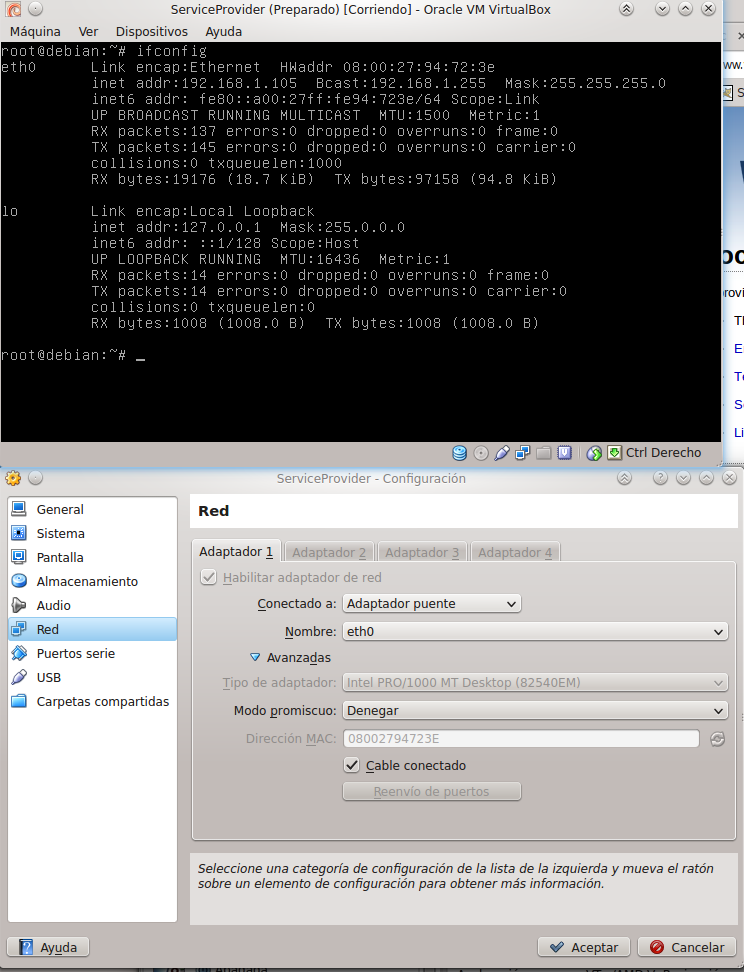
\includegraphics[width=0.7\textwidth]{img/maquinavirtual}
\caption{Maquina virtual ejecutandose en modo bridge.}
\label{fig:vbox}
\end{figure} \newpage
\section{Intercambios entre entidades} \label{sec:intercambio}
Para mostrar un ejemplo de intercambio entre entidades he realizado tres pruebas:
\begin{enumerate}
 \item El cliente pide un recurso al Service Provider y no está autenticado.
 \item El cliente pide un recurso al Service Provider y está autenticado.
 \item El cliente pide un recurso al Service Provider 2 y está autenticado.
\end{enumerate}

Las pruebas se han realizado de manera consecutiva. La correspondencia de las direcciones IP es la siguiente:
\begin{center}
\begin{tabular}{| l | c |}
	\hline
	\textbf{Entidad} & \textbf{IP} \\ \hline \hline 
	Cliente & 192.168.1.12 \\ \hline
	Service Provider & 192.168.1.140 \\ \hline
	Service Provider 2 & 192.168.1.134 \\ \hline
	Identity Provider & 192.168.1.135 \\ \hline
\end{tabular}
\end{center}

\subsubsection*{Primer intercambio}
En la figura \ref{fig:int1} se ve el intercambio número uno. Este consiste en la petición de un recurso al Service Provider sin que el cliente esté autenticado.

\begin{figure}[h!]
\centering
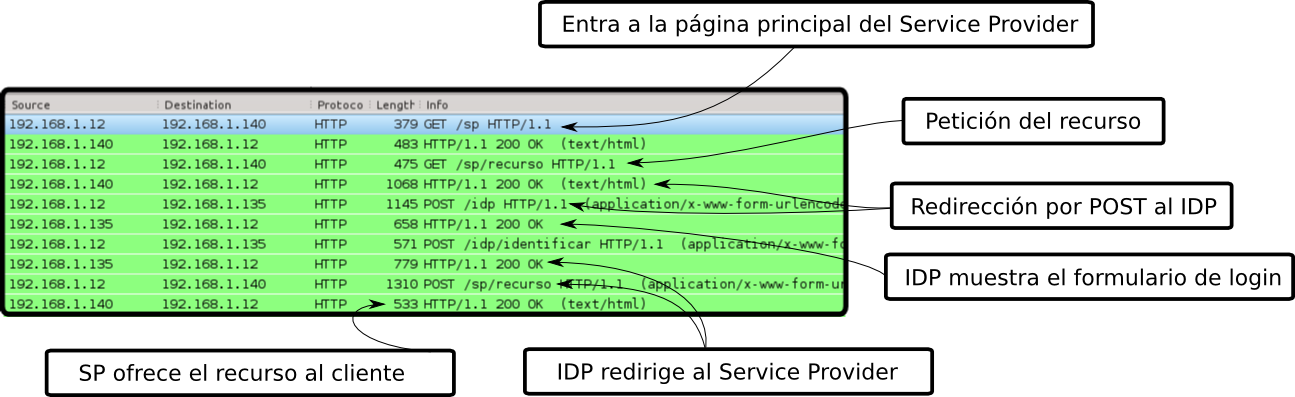
\includegraphics[width=\textwidth]{img/intercambio1-comentado}
\caption{Petición inicial del recurso.}
\label{fig:int1}
\end{figure}

A continuciación describo con detalle el intercambio:
\begin{enumerate}
 \item El cliente entra en la página principal del Service Provider, http://sp.seg.um/sp.
 \item El cliente solicita un recurso protegido.
 \item El Service Provider ve que la sesión del cliente no está autenticada, por lo que emite una página que le redirige al Identity Provider (por el método POST) junto con un Authentication Request.
 \item El cliente reenvía la petición al Identity Provider.
 \item El Identity Provider responde al cliente mostrándole el formulario de autenticación, donde el cliente introduce su usuario y contraseña.
 \item El Identity Provider autentica correctamente al usuario y le redirige al recurso solicitado del Service Provider enviando un Response.
 \item El Service Provider recibe el Response y ve que el usuario fue autenticado correctamente. A partir de ahora, el cliente tiene acceso a los recursos.
 \item El Service Provider ofrece el recurso al cliente.
\end{enumerate}

\subsubsection*{Segundo intercambio}
El segundo intercambio (figura \ref{fig:int2}) consiste en una petición al Service Provider estando ya autenticado el cliente:

\begin{figure}[h!]
\centering
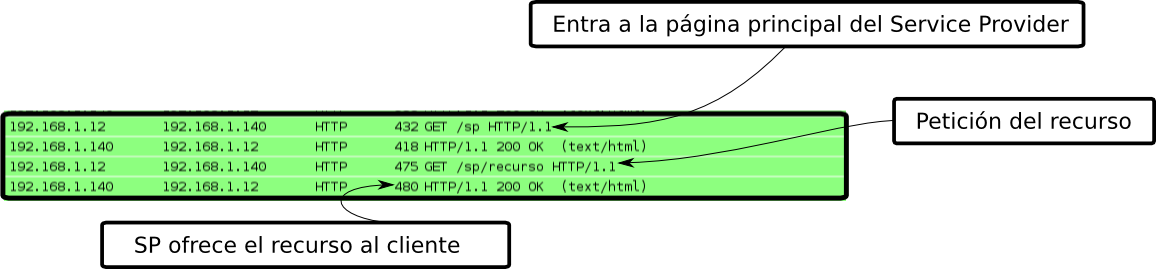
\includegraphics[width=\textwidth]{img/intercambio2-comentado}
\caption{Petición del recurso ya autenticado.}
\label{fig:int2}
\end{figure}

\begin{enumerate}
 \item El cliente entra en la página principal.
 \item El cliente solicita el recurso.
 \item El Service Provider recibe los datos de la sesión del cliente y ve que ya está autenticado en el Identity Provider.
 \item El Service Provider ofrece el recurso directamente al cliente.
\end{enumerate}

\subsubsection*{Tercer intercambio}
El tercer intercambio (figura \ref{fig:int3}) muestra al cliente accediendo a un recurso en otro Service Provider (llamado Service Provider 2).

\begin{figure}[h!]
\centering
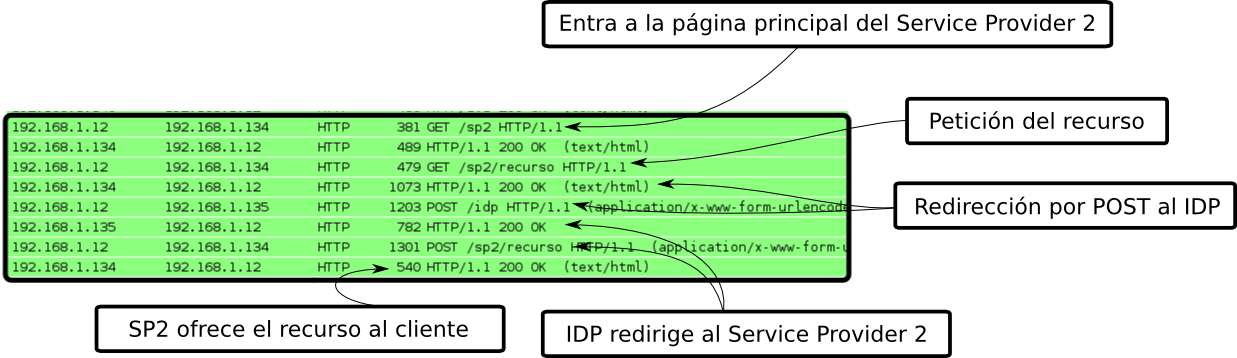
\includegraphics[width=\textwidth]{img/intercambio3-comentado}
\caption{Petición de un recurso en otro Service Provider ya autenticado.}
\label{fig:int3}
\end{figure}

\begin{enumerate}
 \item El cliente, tras acceder a la página principal (http://sp2.seg.um/sp2) solicita acceso al recurso protegido.
 \item El cliente es redirigido por POST al Identity Provider para autenticación, ya que éste no está autenticado en el sistema propio.
 \item El Identity Provider identifica al cliente automáticamente y le considera autenticado.
 \item Reenvía un Response al Service Provider 2.
 \item Service Provider 2 devuelve el recurso.
\end{enumerate}

\begin{figure}[h!]
\centering
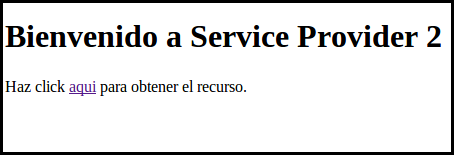
\includegraphics[width=0.6\textwidth]{img/sp2}
\caption{Página inicial del Service Provider 2 sin el cliente autenticado.}
\label{fig:sp2}
\end{figure}
 \newpage
\section{Despliegue}

A continuación se detallan los pasos seguidos para desplegar el escenario:

\begin{enumerate}
 \item Crear tres máquinas virtuales.
 \begin{itemize}
  \item Instalar Tomcat 7 y Oracle Java 7.
  \item No hace falta configurar nada a nivel de red, tan solo saber la IP asignada en caso de modo puente, o el puerto para la traducción en modo NAT.
  \item Instalar el paquete tomcat-manager para gestionar aplicaciones con interfaz web.
 \end{itemize}
 \item Desplegar sitios web.
 \begin{itemize}
  \item Accediendo al manager de Tomcat.
  \item Se suben y despliegan los archivos .war de cada aplicacion en cada máquina virtual.
 \end{itemize}
 \item Configurar el cliente para que los nombres de dominio (descritos en la figura \ref{fig:escenario}) sean resolubles.
 \item Probar el escenario entrando en http://sp.seg.um/sp, por ejemplo. Se pueden seguir los pasos descritos en la sección \ref{sec:intercambio}.
\end{enumerate}

\begin{figure}[h!]
\centering
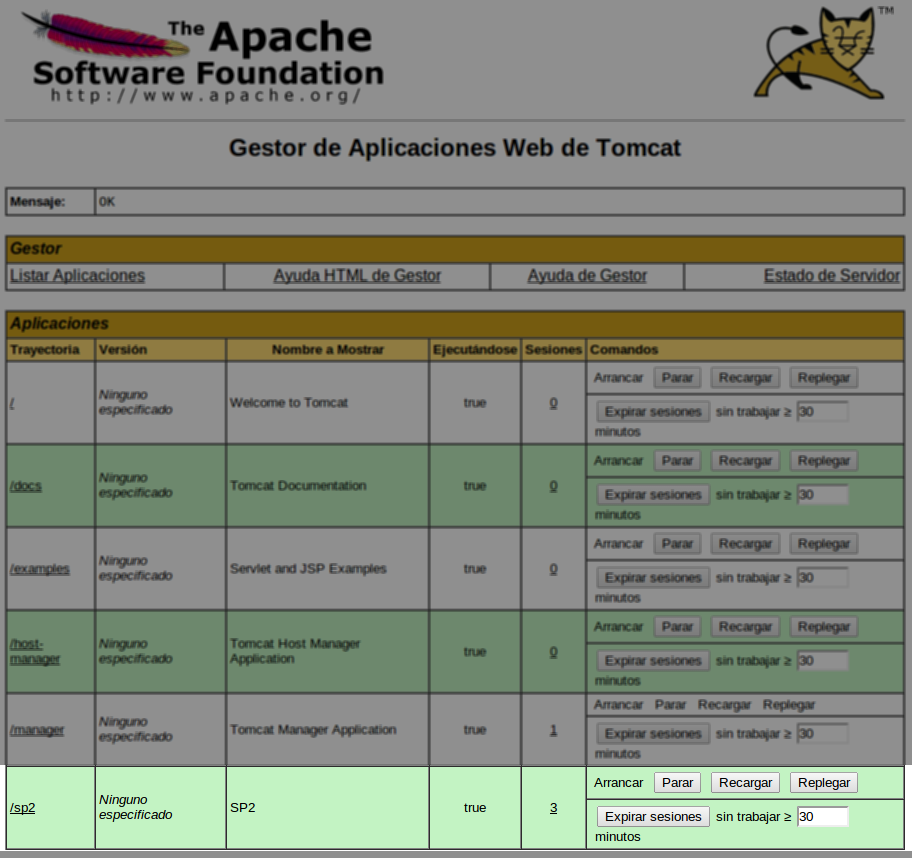
\includegraphics[width=0.9\textwidth]{img/tomcat}
\caption{Tomcat tiene desplegada la aplicacion \emph{sp2} (Service Provider 2).}
\label{fig:tomcat}
\end{figure}

El código está accesible en un repositorio público en Github: \url{https://github.com/LeandroGuillen/SAML.git}. \newpage
%%%%%%%%%%%%%%%%%%%%%%%%%%%%%%%%%%%%%%%%%%%%%%%%%%%
\newpage
% \appendix

\nocite{samlcore}
\nocite{samlprofiles}
\nocite{sureshatt}
\nocite{oracle}
\nocite{sessiontracking}
\nocite{virtualbox}
\nocite{msdn}

% \section{Sobre este documento}
% Elaborado con \LaTeX, Kile, openSUSE 64 bits.

\bibliographystyle{plain}
\bibliography{refs} % mi archivo refs.bib

\end{document}
